\chapter{Descomposición en valores singulares}

\section{Motivación: número de condición y autovalores}

Ya vimos que una matriz cuadrada está mal condicionada si está cerca de una matriz singular. O equivalentemente, está cerca de una matriz que no tiene el máximo rango posible. Podemos extender esta última idea a matrices rectangulares.

La matriz
$$
\Ab = \begin{pmatrix}
1 & 1 \\
1 & 1 \\
1 & 1+ \epsilon \end{pmatrix}
$$
tiene rango 2 si $\epsilon \neq 0$ pero está muy cerca de una matriz de rango 1 si $\epsilon$ es chico.
Podemos pensar intuitivamente que la matriz est\'a ``mal condicionada'', aunque la definición que vimos no se aplica para matrices rectangulares.

\begin{observacion} Para saber si una matriz cuadrada está mal condicionada no alcanza ver que hay un autovalor cercano a 0 o el determinante es chico.
\end{observacion}

\begin{ejemplo} La matriz
$
\Ab = \begin{pmatrix}
\epsilon & 0 & 0 \\
0 & \epsilon & 0 \\
0 & 0 & \epsilon
\end{pmatrix}
$
está bien condicionada para cualquier $\epsilon \neq 0$.
\end{ejemplo}


Relacionamos ahora el número de condición con los autovalores de una matriz.

Para matrices simétricas,
$$
\kappa_2(\Ab) = \|\Ab\|_2 \|\Ab^{-1}\|_2 = |\lambda_{\max{}}(\Ab)| \left|\frac{1}{\lambda_{\min{}}(\Ab)}\right| = \frac{|\lambda_{\max{}}(\Ab)|}{|\lambda_{\min{}}(\Ab)|}.
$$

Vemos que lo que determina que una matriz está mal condicionada es la relación entre el autovalor de mayor módulo y el autovalor de menor módulo.
\section{Introducción}
Comencemos la sección con un experimento numérico. Generemos matrices simétricas al azar y grafiquemos la imagen del círculo unitario por la transformación lineal resultante. Para conseguir figuras uniformes, reescalamos los gráficos de modo que el círculo unitario (en azul) contenga a su imagen (en rojo). El resultado obtenido es esperable. Las imágenes son elípses debido a que cada una de estas matrices posee una base
$\{\vb_1,\vb_2\}$ de autovectores ortonormales. Es decir $\Ab\vb_i=\lambda_i\vb_i$, por lo que cualquier punto $\vb$ del círculo unitario puede escribirse como $\vb=x_1\vb_1+x_2\vb_2$ con $1=x_1^2+x_2^2$, por lo que $A\vb=x_1\lambda_1\vb_1+x_2\lambda_2\vb_2$ es un punto de una elipse de semiejes a lo largo de
las rectas generadas por $\vb_1$ y $\vb_2$ de longitudes $|\lambda_1|$ y $|\lambda_2|$.

\begin{figure}\label{fig:expsimetrico}
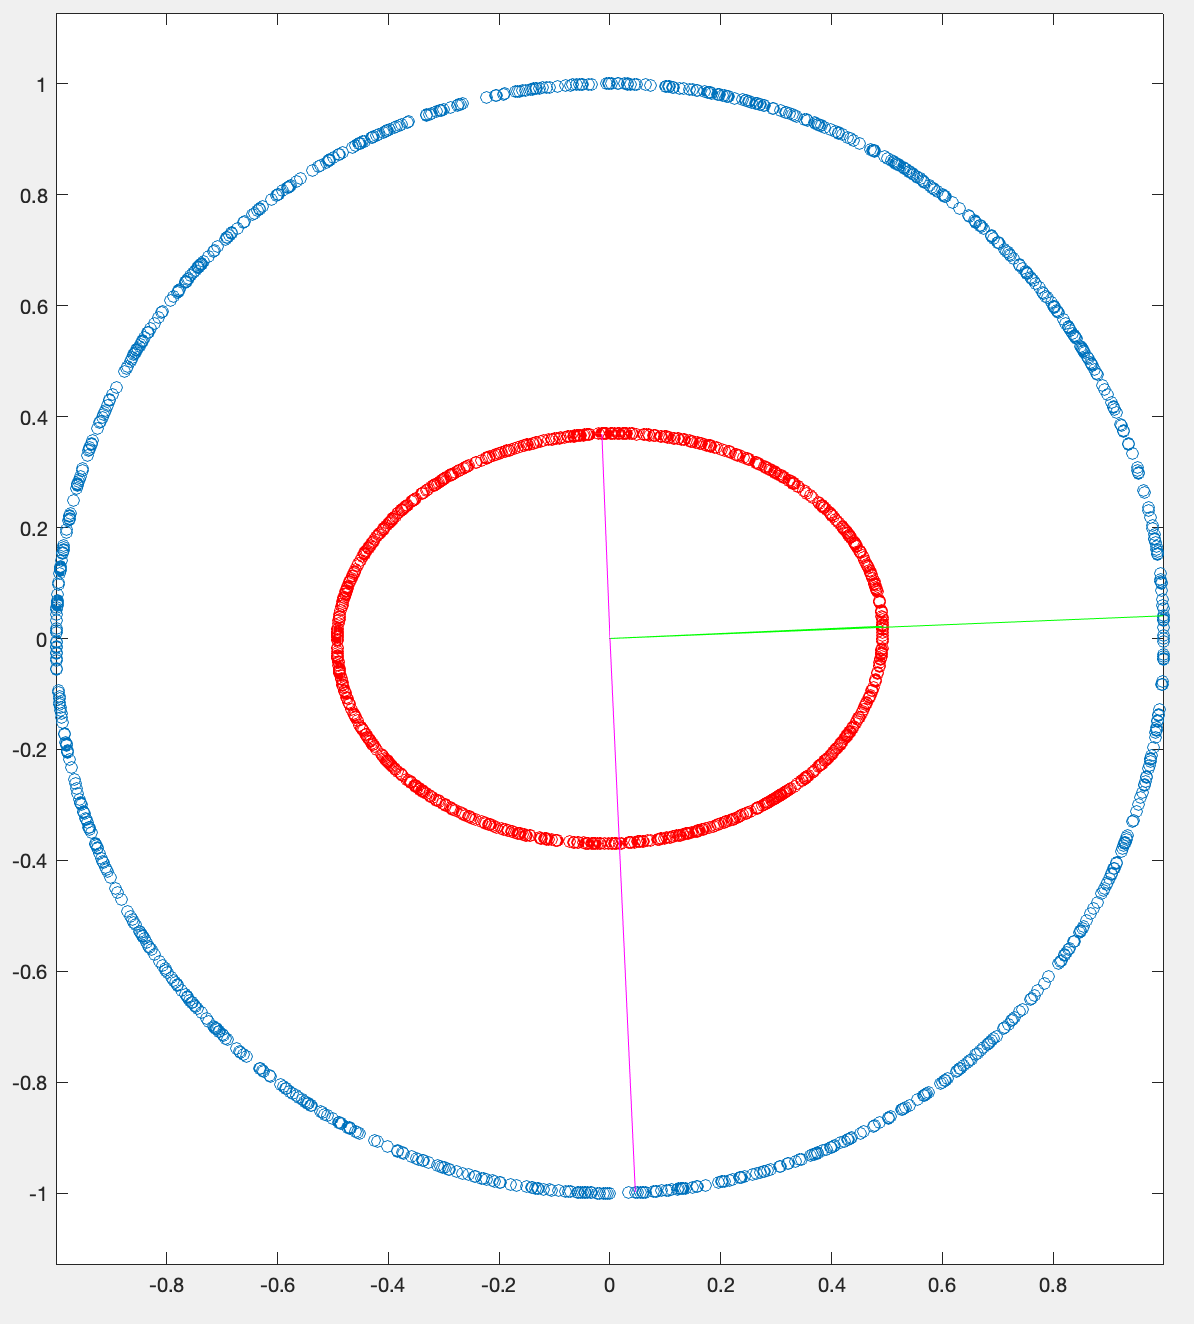
\includegraphics[scale=.15]{randsim1.png}
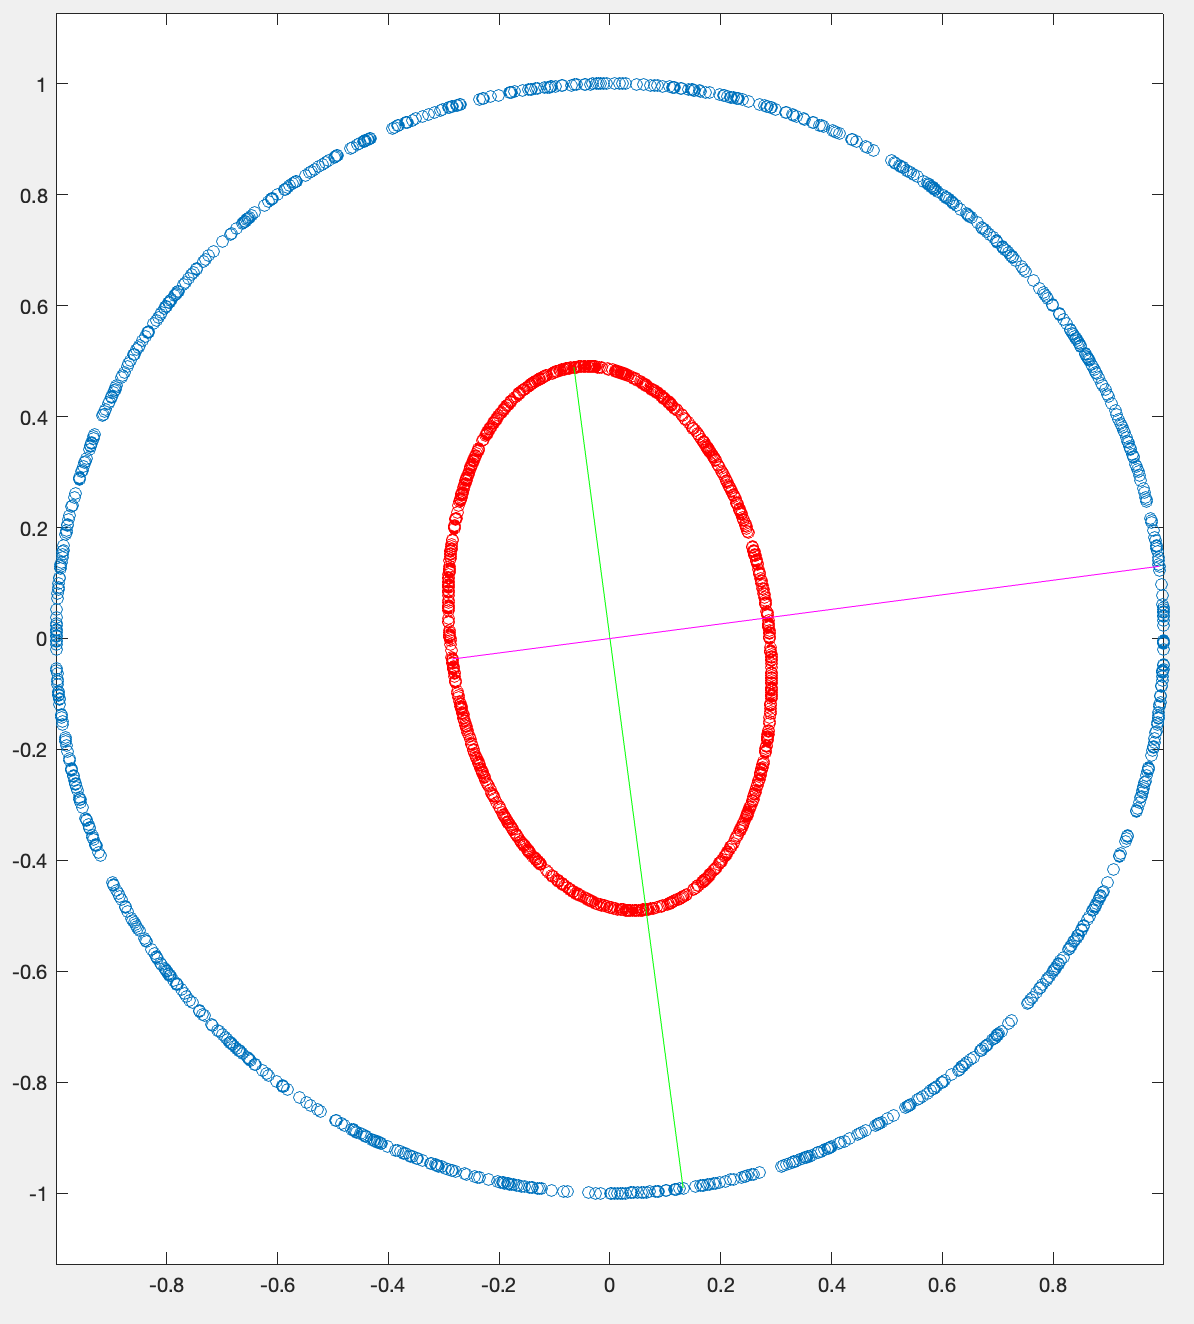
\includegraphics[scale=.15]{randsim2.png}
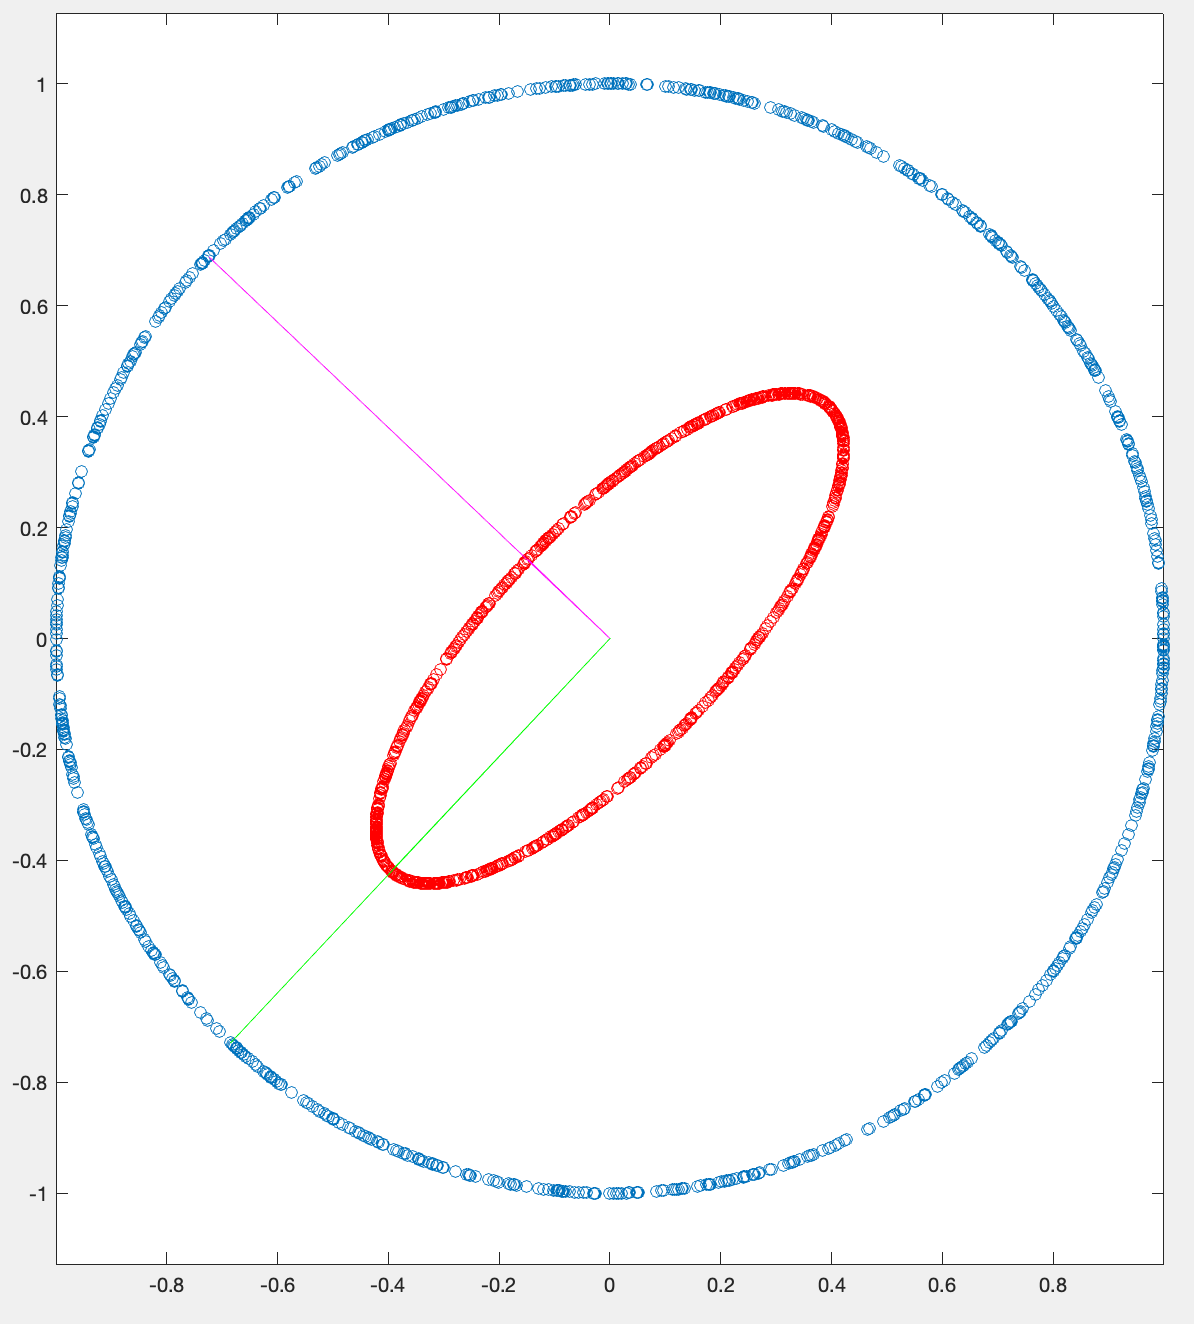
\includegraphics[scale=.15]{randsim3.png}
\caption{Elípses obtenidas por el mapeo del circulo unitario a través de matrices simétricas.}
\end{figure}
Lo extraordinario es que algo similar ocurre con matrices aleatorias cualesquiera, como podemos ver en la Figura \ref{fig:expgral}. En este caso no podemos garantizar una base de autovectores ortonormales, sin embargo podemos estudiar las preimágenes de los semiejes de las elipses (en verde y rosa respectivamente) y notamos que provienen de vectores unitarios ortogonales (con el mismo color en las figuras). Es decir que nuestro experimento sugiere la existencia de dos pares de vectores ortonormales $\{\vb_1,\vb_2\}$
y $\{\ub_1,\ub_2\}$ y dos escalares $\sigma_1,\sigma_2$, que podemos suponer ordenados (i.e. $\sigma_1\ge\sigma_2\ge 0$) y no negativos, cambiando si hicera falta $\ub_i$ por $-\ub_i$, tales que  $\Ab\vb_i=\sigma_i\wb_i$.

Esta observación nos permite escribir
$$
\Ab\Vb=\Ub\Sigmab
$$
donde
$$
\Vb=\begin{pmatrix} \vert &  \vert \\  \vb_1 &  \vb_2 \\ \vert &  \vert \end{pmatrix}\qquad
\Sigmab=\begin{pmatrix} \sigma_1 &  0 \\  0 &  \sigma_2 \end{pmatrix}\qquad
\Ub=\begin{pmatrix} \vert &  \vert \\  \ub_1 &  \ub_2 \\ \vert &  \vert \end{pmatrix}
$$
con matrices $\Vb,\Ub$ ortogonales. Dicho otro modo puede factorizarse $\Ab$ como
$$
\Ab=\Ub\Sigmab\Vb^*.
$$

\begin{figure}\label{fig:expgral}
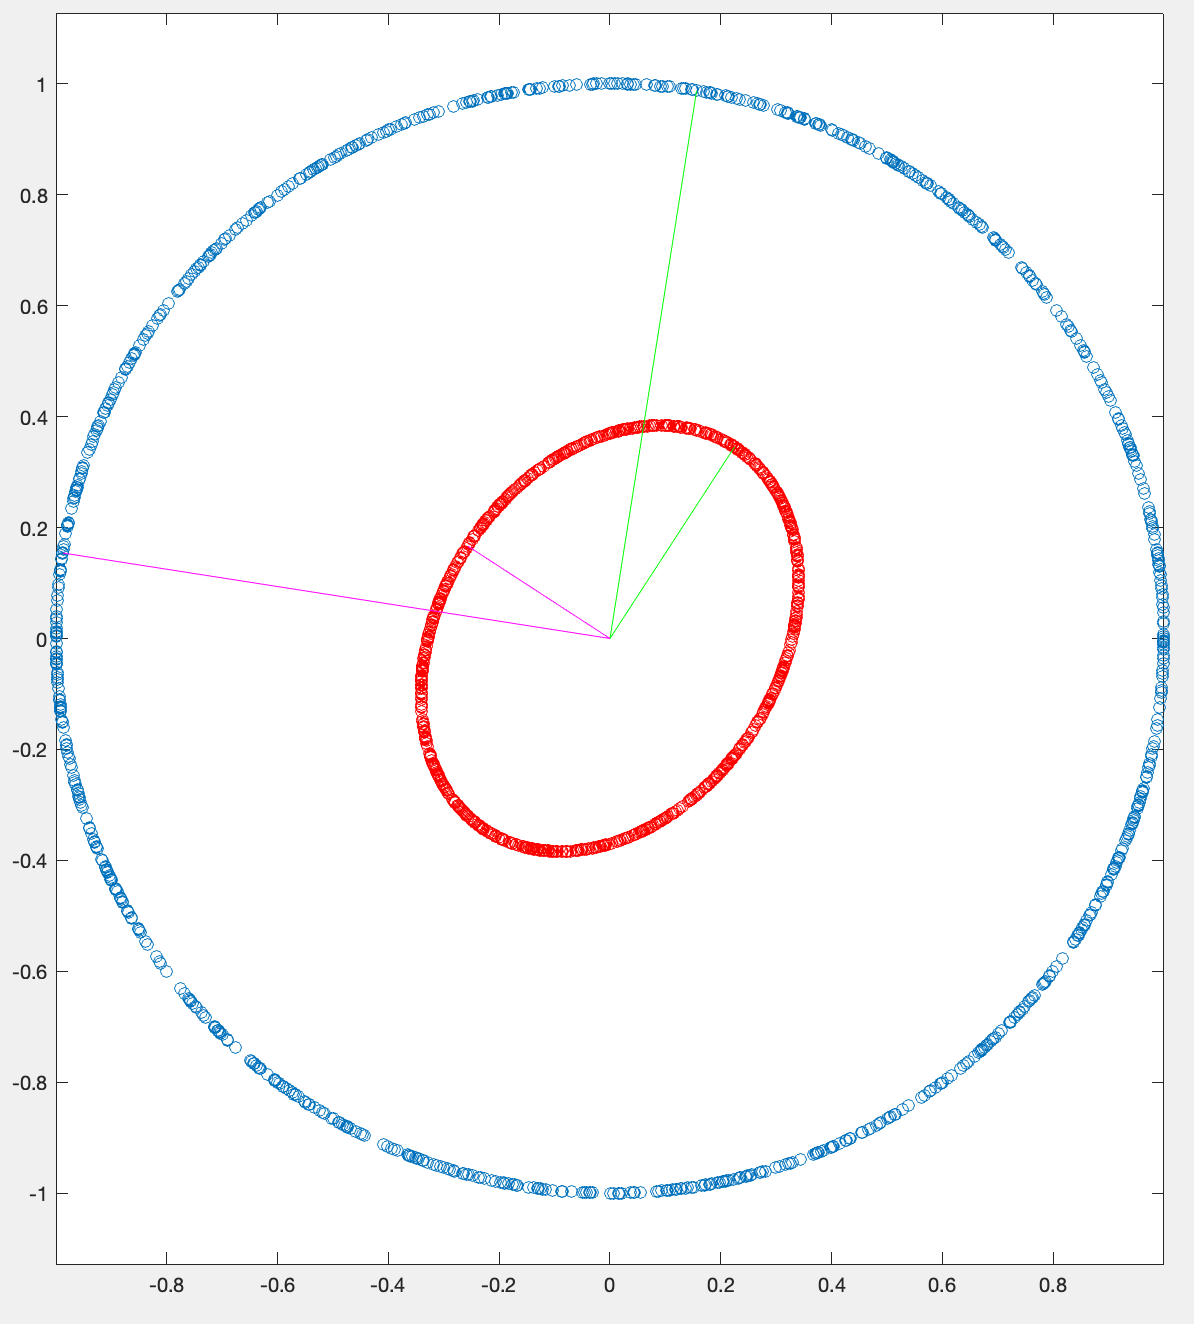
\includegraphics[scale=.15]{rand1.png}
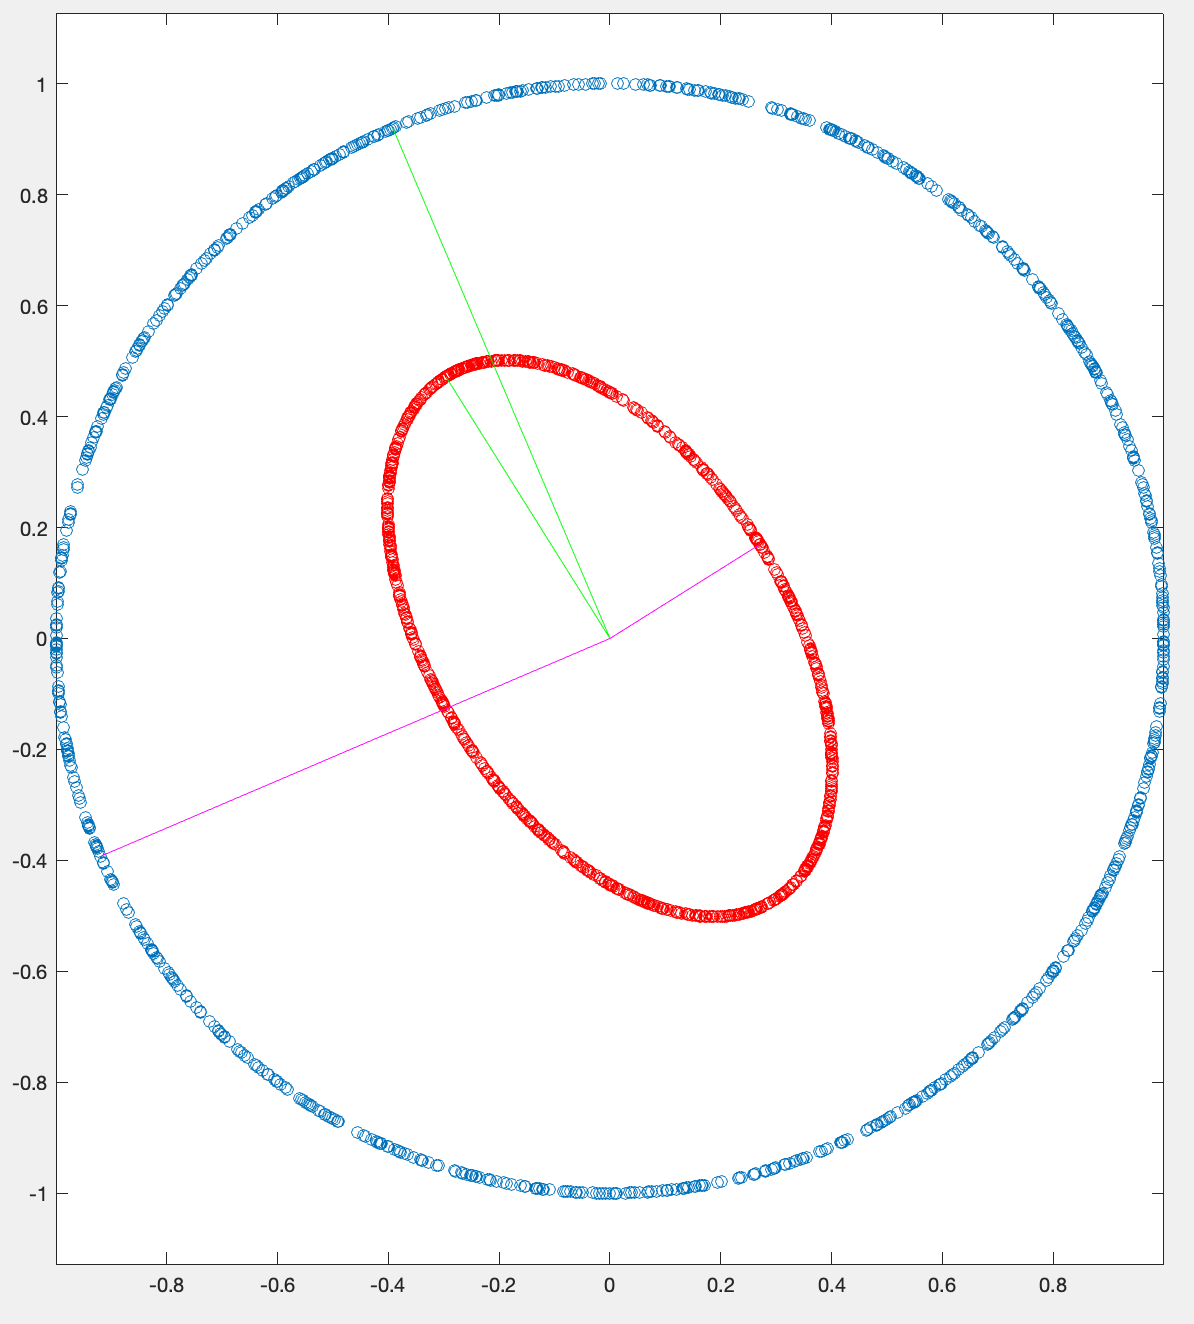
\includegraphics[scale=.15]{rand2.png}
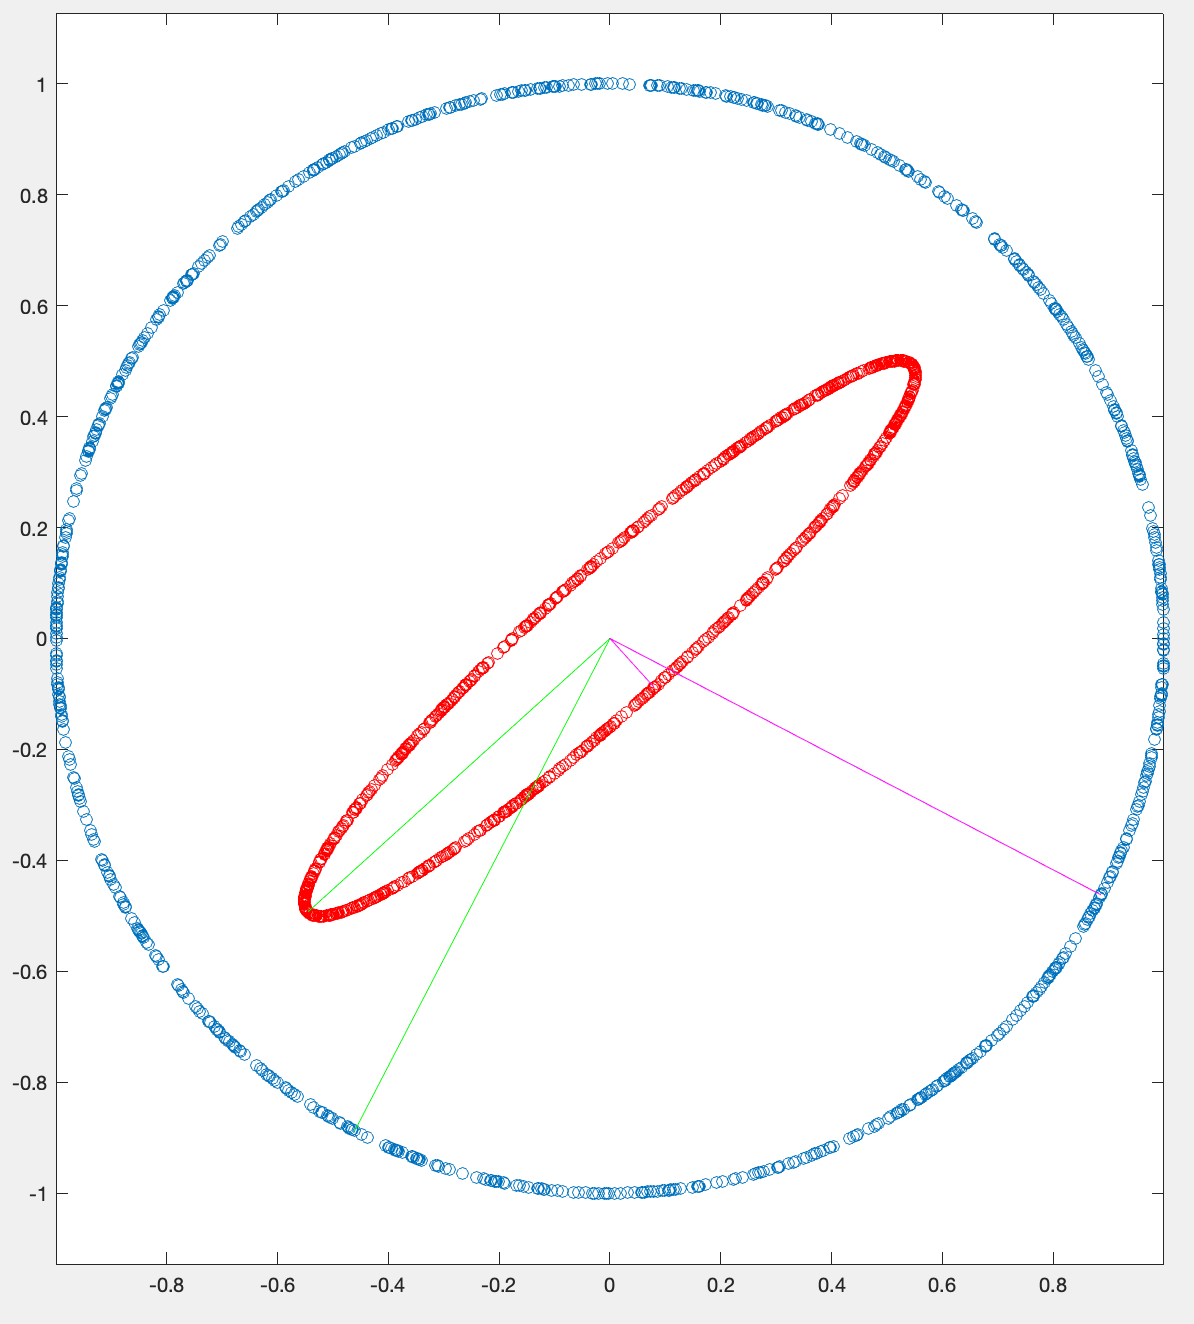
\includegraphics[scale=.15]{rand3.png}
\caption{Elípses obtenidas por el mapeo del circulo unitario a través de matrices generales.}
\end{figure}

\tcc
Esta factorización generaliza en algún sentido a la obtenida al diagonalizar matrices simétricas. Si bien, no toda matriz es diagonalizable en una base ortonormal $\{\vb_1,\vb_2\}$, nuestro experimento dice que algo similar puede obtenerse si nos permiten trabajar con \emph{bases diferentes}: una $\{\vb_1,\vb_2\}$ para el espacio de partida y otra $\{\ub_1,\ub_2\}$ para el de llegada.
\etcc
Lo realmente notable, como veremos en breve, es que esta factorización siempre existe y no solo para matrices cuadradas.
\begin{definicion}
Dada $\Ab \in \K^{m \times n}$, la descomposición en valores singulares SVD es una factorización de $\Ab$
$$\Ab = \Ub \Sigmab \Vb^*,$$
con $\Ub \in \K^{m \times m}$ y $\Vb \in \K^{n \times n}$
matrices unitarias y  $\Sigmab \in \R^{m \times n}$. La matriz $\Sigmab$ tiene la forma
$$
\Sigmab = \begin{pmatrix} \Db \\ \cero_{(m-n) \times n}\end{pmatrix},
$$
si $m \ge n$, o la forma
$$\Sigmab = \begin{pmatrix} \Db & \cero_{m \times (n-m)} \end{pmatrix}$$
si $n > m$. En ambos casos $\Db \in \mathbb{R}^{p \times p}$, donde $p=\min \{m,n\}$, es una matriz diagonal con elementos en
la diagonal $d_{11} \ge d_{22} \ge \dots \ge d_{pp} \ge 0$.
Los elementos no nulos de la diagonal de $\Db$ se denominan \emph{valores singulares} de
$\Ab$, y se notan $\sigma_i(\Ab) = d_{ii}$.
 \end{definicion}

\begin{ejemplo}
$$
\begin{pmatrix}
3 & 2 & 2 \\
2 & 3 & -2 \\
\end{pmatrix} = \begin{pmatrix}
\frac{\sqrt2}{2} & \frac{\sqrt2}{2} \\
\frac{\sqrt2}{2} & -\frac{\sqrt2}{2}
\end{pmatrix} \begin{pmatrix}
5 & 0 & 0 \\
0 & 3 & 0
\end{pmatrix}
\begin{pmatrix}
\frac{\sqrt2}{2} & \frac{\sqrt2}{2} & 0 \\
\frac{\sqrt2}{6} & -\frac{\sqrt2}{6} & \frac{2\sqrt2}{3} \\
\frac23 & -\frac23 & -\frac13
\end{pmatrix}
$$
\end{ejemplo}

\section{Construcción}

Para constuir la descomposición SVD observamos las siguientes relaciones.

Dada una matriz $\Ab \in \K^{m \times n}$, si $\Ab = \Ub \Sigmab \Vb^*$:

\begin{itemize}
\item $\Ab \Ab^* = (\Ub \Sigmab \Vb^*) (\Vb \Sigmab^* \Ub^*) = \Ub (\Sigmab \Sigmab^*) \Ub^*$, con $\Sigmab \Sigmab^* \in \R^{m \times m}$ diagonal.
\item $\Ab^* \Ab = (\Vb \Sigmab^* \Ub^*) (\Ub \Sigmab \Vb^*) = \Vb (\Sigmab^* \Sigmab) \Vb^*$, con $\Sigmab^* \Sigmab \in \R^{n \times n}$ diagonal.
\end{itemize}

Recordar que $\Ab^* \Ab$ y $\Ab \Ab^*$ son matrices semidefinidas positivas y por
lo tanto diagonalizables con autovalores no-negativos y base ortonormal
de autovectores.

En base a estas relaciones, concluimos:
\begin{itemize}
\item  Las columnas de $\Ub$ son una base de autovectores de
    $\Ab \Ab^* \in \K^{m \times m}$.

\item Las columnas de $\Vb$ son una base autovectores de
    $\Ab^* \Ab \in \K^{n \times n}$.

\item Los valores singulares en $\Sigmab$ son la raíz cuadrada de los
    autovalores no nulos de $\Ab^* \Ab$ o $\Ab \Ab^*$ ordenados de mayor a menor.
\end{itemize}


Esto nos da un método para calcular la descomposición. 

Primero construimos la matriz $\Vb$ tomando una base de autovectores de $\Ab^* \Ab$.

Luego obtenemos las filas de $\Ub$ a partir de la relación
$$
\Ab = \Ub \Sigmab \Vb^*
$$
multiplicando por $\Vb$:
$$
\Ab \Vb = \Ub \Sigmab.
$$

En el término de la izquierda tenemos
$$
\Ab\Vb = \begin{pmatrix} \vert & & \vert \\ \Ab \vb_1 & \dots & \Ab \vb_n \\ \vert & & \vert \end{pmatrix}.
$$



\subsection{Si $m \le n$}
Si $m \le n$,
$$
\Ab \Vb = \Ub \Sigmab = \begin{pmatrix}  \vert & & \vert \\ \ub_1 & \dots & \ub_m \\ \vert & & \vert \end{pmatrix}
\begin{pmatrix} \begin{array}{ccc|c@{\mskip5mu}}\sigma_1 & & \\ & \ddots & & \text{\Large 0}           \\ & & \sigma_m\end{array}\\      \end{pmatrix} = \begin{pmatrix}
\begin{array}{ccc|c@{\mskip5mu}}\vert & & \vert \\ \sigma_1 \ub_1 & \dots & \sigma_m \ub_m & \text{\Large 0}           \\ \vert & & \vert \end{array}\\
 \end{pmatrix}
$$

Por lo tanto, para $1 \le i \le n$, las columnas de $\Ub$ cumplen $\sigma_i \ub_i = \Ab \vb_i$, donde
$\vb_i$ son las columnas de $\Vb$. Obtenemos
$$
\ub_i = \frac{1}{\sigma_i} \Ab \vb_i.
$$
para $1 \le i \le m$ y $\sigma_i \neq 0$.
Si existen valores singulares nulos, las columnas correspondientes de $\Ub$ las elegimos completando una base ortonormal $\{\ub_1, \dots, \ub_m\}$ de $\K^{m \times m}$.

\subsection{Si $m > n$}

Si $m \ge n$,
$$
\Ab \Vb = \Ub \Sigmab =  \begin{pmatrix} \vert & & \vert \\ \ub_1 & \dots & \ub_m \\ \vert & & \vert \end{pmatrix}
\left(\begin{array}{ccc}\sigma_1 & & \\ & \ddots & \\ & &  \sigma_n\\\hline         & \rule{0cm}{15pt} \text{\Large 0} &
 \end{array}\right) = \begin{pmatrix} \vert & & \vert \\ \sigma_1 \ub_1 & \dots & \sigma_n \ub_n \\ \vert & & \vert \end{pmatrix}
$$

Por lo tanto, para $1 \le i \le n$, las columnas de $\Ub$ cumplen $\sigma_i \ub_i = \Ab \vb_i$, donde
$v_i$ son las columnas de $\Vb$. Obtenemos
$$
\ub_i = \frac{1}{\sigma_i} \Ab \vb_i.
$$
para $1 \le i \le n$ y $\sigma_i \neq 0$.
El resto de las columnas de $\Ub$ las elegimos completando una base ortonormal $\{\ub_1, \dots, \ub_m\}$ de $\K^{m \times m}$.

\begin{ejercicio}
Calcular la descomposición SVD de la matriz
$$
\Ab = \begin{pmatrix}
3 & 2 & 2 \\
2 & 3 & -2 \\
\end{pmatrix} \in \R^{2 \times 3}.
$$
realizando los siguientes pasos:
\begin{enumerate}
\item Construir la matriz $\Vb$ tomando como columnas una base ortonormal de autovectores de $\Ab^* \Ab \in \R^{3 \times 3}$.
\item Calcular los valores singulares $\sigma_i = \sqrt{\lambda_i}$, $i = 1,2$, con $\lambda_i$ los autovalores (no nulos) de $\Ab^* \Ab$.
\item Calcular las columnas de $\Ub$ por la fórmula $\ub_i = \frac{1}{\sigma_i} \Ab \vb_i$, $i = 1,2$.
\item Verificar.
\end{enumerate}
\end{ejercicio}

Ya vimos cómo construir una descomposición SVD. Si repasamos la construcción que realizamos, vemos que utilizamos la existencia de tal descomposición para obtener propiedades de las matrices en la descomposición. Para probar la existencia de la descomposición nos falta completar algunos detalles de la construcción.

\begin{teo}
Dada una matriz rectangular $\Ab \in \K^{m \times n}$, existen matrices
\begin{itemize}
\item $\Ub \in \K^{m \times m}$ unitaria,
\item $\Sigmab \in \R^{m \times n}$, con $\Sigmab = (\Db | 0)$ o $\Sigmab = \left(\frac{\Db}{0}\right)$, $\Db$ diagonal y $d_{11} \ge \dots \ge d_{ss} \ge 0$ ($s = \min\{m,n\}$),
\item $\Vb \in \K^{n \times n}$ unitaria,
\end{itemize}
tales que $\Ab = \Ub \Sigmab \Vb^*$.
Los valores no nulos $d_{11} \ge \dots \ge d_{ss} > 0$ son \'unicos y se denominan \emph{valores singulares} de $\Ab$, $\sigma_i = d_{ii}$.
\end{teo}

\begin{proof}
En la construcción que hicimos, falta ver que los vectores $\ub_i = \frac{1}{\sigma_i} \Ab \vb_i$ construidos son ortogonales. Calculamos

$$
\begin{aligned}
\ub_j^* \ub_i &= \left(\frac{1}{\sigma_j} \vb_j^* \Ab^* \right) \left(\Ab \vb_i  \frac{1}{\sigma_i}\right) \\
&= \frac{1}{\sigma_j} \vb_j^* ( \Ab^* \Ab) \vb_i  \frac{1}{\sigma_i} = \frac{1}{\sigma_j} (\vb_j^*) ( \Vb \Sigmab^* \Sigmab \Vb^*) \vb_i  \frac{1}{\sigma_i}
\end{aligned}
$$
y usando que $\Vb^* \vb_i = \eb_i$, obtenemos
$$
\ub_j^* \ub_i = \frac{1}{\sigma_j} (\eb_j^* \Sigmab^*) (\Sigmab \eb_i)  \frac{1}{\sigma_i}
 = \frac{1}{\sigma_j} (\sigma_j \eb_j^*) ( \sigma_i \eb_i)  \frac{1}{\sigma_i} = \eb_j^* \eb_i
 = \begin{cases} 1 & \text{ si } i = j \\
 0 & \text{ si } i \neq j
 \end{cases}
$$
\end{proof}

\section{Valores singulares y norma-2}

Ahora estamos en condiciones de retomar la discusión inicial de este cápítulo.

\begin{teo}
Dada una matriz rectangular $\Ab \in \K^{m \times n}$,
$$
\|\Ab\|_2 = \sigma_1(\Ab).
$$
\end{teo}

\begin{proof}
 Recordando que multiplicar por una matriz unitaria es una transformación inversible que no cambia la norma de un vector,
$$
\begin{aligned}
\|\Ab\|_2 &= \sup_{\|\xb\|_2 = 1} \|\Ab\xb\|_2 \\
& = \sup_{\|\xb\|_2 = 1} \|\Ub \Sigmab \Vb^* \xb\|_2 = \sup_{\|\xb\|_2 = 1} \|\Sigmab \Vb^* \xb\|_2 \\
&= \sup_{\|\yb\|_2 = 1} \|\Sigmab \yb \|_2  = \sup_{\|\yb\|_2 = 1} (\sum_{i=1}^r \sigma_i^2 |y_i|^2)^{\frac12} \le \sigma_1
\end{aligned}
$$
\end{proof}

\begin{proposicion} Si $\Ab \in \K^{m \times n}$ y $\rank(\Ab) = n$, entonces
$$
\min_{\|x\|_2=1} \|\Ab\|_2 = \sigma_n(\Ab)
$$
\end{proposicion}

\begin{corolario}
Si $\Ab \in \K^{n \times n}$ inversible,
$$
\cond_2(\Ab) = \frac{\sigma_1(\Ab)}{\sigma_n(\Ab)}.
$$
\end{corolario}

En general, para cualquier matriz $\Ab \in \K^{m \times n}$ rectangular de rango máximo, definimos $$\cond_2(\Ab) = \frac{\sigma_1(\Ab)}{\sigma_r(\Ab)},$$
con $r = \min\{m,n\}$.

\section{Distancia a matrices de menor rango}

Por último, vemos cómo formalizar la noción de matrices rectangulares mal condicionadas o cercanas a matrices de menor rango.

Dada una matriz $\Ab \in \K^{n \times n}$, buscamos una matriz singular lo más cercana posible a $\Ab$.
En otras palabras, buscamos $\Bb \in \K^{n \times n}$ de norma lo más chica posible tal que $\Ab + \Bb$ sea singular.

\begin{enumerate}
\item $\Ab + \Bb = \Ab (\Ib + \Ab^{-1} \Bb)$
\item Si $\|\Ab^{-1}\Bb\| < 1$, entonces $\Ib + \Ab^{-1}\Bb$ (y por lo tanto $\Ab+\Bb$) es inversible.
\item Por lo tanto, si $\Ab + \Bb$ es singular y $\Ab$ es inversible, debe ser $\|\Bb\| \ge 1 / \|\Ab^{-1}\|$.
\item Tomando norma-2, y $\Ab = \Ub \Sigmab \Vb^*$ la SVD, $\|\Ab^{-1}\|_2 = 1/\sigma_n$.
\item Por lo tanto, si $\Ab+\Bb$ es singular, debe ser $\|\Bb\| \ge \sigma_n(\Ab)$.
\item Podemos tomar $\Bb = \Ub \Eb \Vb^*$, con $\Eb = \diag(0, 0, \dots, 0, -\sigma_n)$, que cumple $\|\Bb\|_2 = \|\Eb\|_2 = \sigma_n$.
\end{enumerate}

\begin{teo}
Dada $\Ab \in \K^{n \times n}$ inversible, con $\Ab = \Ub \Sigmab \Vb^*$ su descomposición en valores singulares.
Definiendo
{\small
$$\Sigmab_{n-1} =
\begin{pmatrix}
\sigma_1 & & & \\
 & \ddots & & \\
 & & \sigma_{n-1} & \\
 & &  & 0
\end{pmatrix},
$$
}
la matriz $\tilde \Ab = \Ub \Sigmab_{n-1} \Vb^*$ es la matriz singular m\'as cercana a $\Ab$ en norma-2.
\end{teo}

\begin{ejercicio}
Encontrar la matriz singular más cercana a $\Ab = \begin{pmatrix} 1 & 2 & 3 \\ 1 & 3 & 5 \\ 1 & 5 & 8\end{pmatrix}$.
\end{ejercicio}

Podemos ahora el resultado anterior para calcular las matrices más cercanas de distinto rango.

\begin{teo}
Sea $\Ab \in \K^{m \times n}$ de rango $k > 0$, con $\Ab = \Ub \Sigmab \Vb^*$ su descomposición en valores singulares. La matriz $\Ab_1 \in \K^{m \times n}$ de rango $k_1 < k$ más cercana a $\Ab$ en la norma 2 o norma Frobenius es $\Ab_1 = \Ub \Sigmab_{1} \Vb^*$, con
$$\Sigmab_{1} =
\begin{pmatrix}
\sigma_1 & & & \\
 & \ddots & & \\
 & & \sigma_{k_1} & \\
 & &  & 0
\end{pmatrix},
$$
la matriz igual a $\Sigmab$ excepto que solo se usan los valores singulares $\sigma_1, \dots, \sigma_{k_1}$ y los demás se reemplazan por 0.
\end{teo}


\section{Aplicaciones}

\subsection{Reducción de dimensionalidad}

Para una población de $m$ individuos analizamos $n$ variables (features), con $m > n$, y queremos ver si hay variables redundantes o si podemos reducir la cantidad de variables sin perder mucha información.

Dada una matriz $\Ab \in \R^{m \times n}$, $m > n$, el $k$-\'esimo valor singular nos dice la distancia de $\Ab$ a una matriz de rango $k-1$.
Es decir, mide ``cuánta información'' vamos a perder si utilizamos $k-1$ variables en lugar de las $n$ variables originales.

\begin{ejercicio}
Para la siguiente matriz, calcular los valores singulares. ¿Considera que hay variables redundantes? ¿Cuáles variables eliminaría?
\begin{center}
 \begin{tabular}{||c c c c c||}
 \hline
  & $x_1$ & $x_2$ & $x_3$ & $x_4$ \\ [0.5ex]
 \hline\hline
 1 & 100 & 100 & 757  & 220\\
 \hline
 2 & 70 & 80 & 603 & 174 \\
 \hline
 3 & 50 & 90 & 700 & 190 \\
 \hline
 4 & 150 & 40 & 250 & 110 \\
 \hline
 5 & 80 & 10 & 42 & 36 \\ [1ex]
 \hline
\end{tabular}
\end{center}
\end{ejercicio}

\subsection{La pseudo-inversa}

A partir de la descomposición en valores singulares $\Ab = \Ub \Sigma \Vb^*$,
construimos la pseudo inversa de $\Ab$,
$$
\Ab^\dagger = \Vb \Sigmab^\dagger \Ub^*,
$$ 
donde $\Sigmab^\dagger$ se obtiene a partir de $\Sigmab$ transponiéndola y
reemplazando los elementos no nulos $d_{ii}$ en la diagonal por
$1 / d_{ii}$.

\begin{ejercicio} Calcular la pseudo-inversa de
$$
\begin{pmatrix}
3 & 2 & 2 \\
2 & 3 & -2 \\
\end{pmatrix} = \begin{pmatrix}
\frac{\sqrt2}{2} & \frac{\sqrt2}{2} \\
\frac{\sqrt2}{2} & -\frac{\sqrt2}{2}
\end{pmatrix} \begin{pmatrix}
5 & 0 & 0 \\
0 & 3 & 0
\end{pmatrix}
\begin{pmatrix}
\frac{\sqrt2}{2} & \frac{\sqrt2}{2} & 0 \\
\frac{\sqrt2}{6} & -\frac{\sqrt2}{6} & \frac{2\sqrt2}{3} \\
\frac23 & -\frac23 & -\frac13
\end{pmatrix}
$$
\end{ejercicio}

Se cumplen las siguientes propiedades.

\begin{proposicion}\leavevmode
\begin{itemize}
\item $\Ab \Ab^\dagger \Ab = \Ab$ y $\Ab^\dagger \Ab \Ab^\dagger = \Ab^\dagger$ (pero en general no se cumple
    $\Ab \Ab^\dagger = I_m$ o $\Ab^\dagger \Ab= I_n$)
\item Si $\Ab \in \mathbb{K}^{n \times n}$ es inversible, $\Ab^{-1} = \Ab^\dagger$.
\end{itemize}
\end{proposicion}

\begin{proof} Ejercicio.
\end{proof}

\begin{ejercicio} Verificar $\Ab \Ab^\dagger \Ab = \Ab$ para $\Ab = \begin{pmatrix}
3 & 2 & 2 \\
2 & 3 & -2 \\
\end{pmatrix}$
\end{ejercicio}

\subsection{Resolución de sistemas de ecuaciones}

Enunciamos ahora el resultado principal, cuya demostración veremos en la Práctica 6 de Mínimos Cuadrados.
\begin{teo}
Dada la ecuación $\Ab \xb = \bb$, con $\Ab \in \mathbb{\K}^{m \times n}$, si el
sistema tiene soluciones entonces
$$
\zb = \Ab^\dagger \bb
$$
es una solución y si hay infinitas soluciones, $\zb$ es la solución de
mínima norma-2.
\end{teo}

Utilizando la pseudo-inversa podemos obtener también un criterio para determinar si un sistema tiene solución.


\begin{teo}
El sistema $\Ab \xb = \bb$ tiene solución si y solo si $\Ab \Ab^\dagger \bb = \bb$.
\end{teo}

\begin{proof}\leavevmode
\begin{itemize}
\item Si $\Ab \Ab^\dagger \bb = \bb$ entonces $\vb = \Ab^\dagger \bb$ es solución del sistema.
\item Recíprocamente, si existe $\vb$ tal que $\Ab \vb = \bb$, entonces
$$\bb = \Ab \vb = \Ab \Ab^\dagger \Ab \vb = \Ab \Ab^\dagger \bb$$
(aunque usted no lo crea!).
\end{itemize}
\end{proof}

Cuando el sistema solución, la pseudo-inversa nos permite también hallar todas las soluciones.

\begin{teo}
Dadas $\Ab \in \K^{m \times n}$ y $\bb \in \K^n$. Si $\Ab \Ab^\dagger \bb = \bb$, todos los vectores de la forma
$$
\xb = \Ab^\dagger \bb + (\Ib_n - \Ab^\dagger \Ab) \yb
$$
con $\yb \in \K^n$ son soluciones del sistema $\Ab \xb = \bb$.

Más aún, cualquier solución la puedo escribir de esa forma.

\end{teo}

\begin{proof} Si $\xb$ es de esa forma,
$$\begin{aligned}
\Ab \xb &= \Ab(\Ab^\dagger \bb+ (\Ib_n - \Ab^\dagger \Ab) \yb) \\
&= (\Ab\Ab^\dagger \bb) + (\Ab - \Ab\Ab^\dagger \Ab) \yb \\
&= \bb + (\Ab - \Ab) \yb = \bb.
\end{aligned}$$

Ahora, dado un vector $\zb \in \K^n$ tal que $\Ab \zb = \bb$, escribimos
$$
\zb = (\Ab^\dagger \Ab)\zb + (\Ib_n - \Ab^\dagger \Ab) \zb = \Ab^\dagger \bb + (\Ib_n - \Ab^\dagger \Ab) \zb
$$
que es un vector de la forma buscada.

\end{proof}

\begin{observacion}\leavevmode
\begin{itemize}
\item Puede haber soluciones repetidas entre las soluciones obtenidas de esta forma.
\item En particular, el sistema $\Ab \xb = \bb$ tiene solución única si y solo si $\Ab^\dagger \Ab = \Ib_n$.
\end{itemize}
\end{observacion}

\begin{ejercicio} Determinar cuántas soluciones tienen los siguientes sistemas de ecuaciones, y hallar una solución cuando sea posible.
$$
\left\{\begin{array}{rl}x - 2y &= 2\\2x +  y & =1\\x + 3y & = -1\end{array}\right.
\quad \quad \quad
\left\{\begin{array}{rl}x - 2y + z &= 2\\2x +  y + 5z& =1\\x + 3y + 4z& = -1\end{array}\right.
\quad \quad \quad
\left\{\begin{array}{rl}x - 2y + z &= 2\\2x +  y + 5z& =1\\x + 3y + 4z& = 7\end{array}\right.
$$

En \python puede utilizar \texttt{np.linalg.pinv} para calcular la pseudo-inversa.
\end{ejercicio}

\subsection{Compresión de imágenes}

Veamos como comprimir una imagen aplicando reducción de dimensionalidad por SVD.

Tomamos una matriz $\Ab \in \R^{m \times n}$, con $a_{ij} \in [0,1]$, que representa una tonalidad de gris, siendo $0 = $ negro y $1 = $ blanco.

\begin{ejemplo}
Para representar la imagen de la figura, tomamos $\Ab \in \R^{25 \times 15}$.

\begin{center}
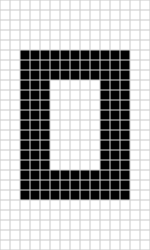
\includegraphics[scale=1.5]{svdO.png}
\end{center}

¿Cuál es el rango de $\Ab$? ¿Cuántos valores singulares no nulos tiene $\Ab$?

\textbf{Eliminamos columnas de $\Ub$}

La descomposición en valores singulares de  $\Ab \in \R^{25 \times 15}$,
$$
\Ab = \Ub \Sigmab \Vb^*
$$
tiene 3 valores singulares no nulos, $\Ub \in \R^{25 \times 25}$, $\Sigmab \in \R^{25 \times 15}$ y $\Vb \in \R^{15 \times 15}$.

¿Podemos descartar filas de $\Ub$ y $\Vb$ sin perder información?

Recordando que
$$
\Ub \Sigmab =  \begin{pmatrix} \vert & & \vert \\ \ub_1 & \dots & \ub_{25} \\ \vert & & \vert \end{pmatrix}
\left(\begin{array}{ccc}\sigma_1 & & \\ & \ddots & \\ & &  \sigma_{15}\\\hline         & \rule{0cm}{15pt} \text{\Large 0} &
 \end{array}\right) = \begin{pmatrix} \vert & & \vert \\ \sigma_1 \ub_1 & \dots & \sigma_{15} \ub_{15} \\ \vert & & \vert \end{pmatrix}
$$
vemos que podemos tomar siempre $\ub_i = \cero$ para $i > 16$ sin perder información, y en nuestro caso también $\ub_i = \cero$ para $i > 3$.

\textbf{Eliminamos columnas de $\Vb$}

Análogamente, a partir de $(\Sigmab \Vb^*)^* = $
$$
\Vb \Sigmab^* = \begin{pmatrix}  \vert & & \vert \\ \vb_1 & \dots & \vb_{15} \\ \vert & & \vert \end{pmatrix}
\begin{pmatrix} \begin{array}{ccc|c@{\mskip5mu}}\sigma_1 & & \\ & \ddots & & \text{\Large 0}           \\ & & \sigma_{15}\end{array}\\      \end{pmatrix} = \begin{pmatrix}
\begin{array}{ccc|c@{\mskip5mu}}\vert & & \vert \\ \sigma_1 \vb_1 & \dots & \sigma_{15} \vb_{15} & \text{\Large 0}           \\ \vert & & \vert \end{array}\\
 \end{pmatrix}
$$
vemos que podemos tomar $\vb_j = \cero$ para $j > 3$ sin perder información.

En forma más compacta, para no guardar tantos 0's, podemos guardar la descomposición
$$
\underset{25 \times 15}\Ab = \underset{25 \times 3}{\begin{pmatrix}  \vert & & \vert \\ \ub_1 & \dots & \ub_{3} \\ \vert & & \vert \end{pmatrix}}
\underset{3 \times 3}{\begin{pmatrix}  \sigma_1 & 0 & 0 \\
0 & \sigma_2 & 0 \\
0 & 0 & \sigma_3  \end{pmatrix}}
\underset{3 \times 15}{\begin{pmatrix}
- \vb_1 - \\
- \vb_2 - \\
- \vb_3 - \\
\end{pmatrix}}
$$

\textbf{Cantidad de datos}

En total, necesitamos guardar:
\begin{itemize}
\item 3 columnas de $\Ub \rightarrow 75$ valores
\item 3 columnas de $\Vb \rightarrow 45$ valores
\item 3 valores singulares
\item Total: $75 + 45 + 3 = 123$ valores
\end{itemize}

Para guardar la matriz original necesitamos $25 \times 15 = 375$ valores

\end{ejemplo}

Veamos otro ejemplo más realista.

\begin{ejemplo}

Tomamos ahora la imagen de un \'arbol $\Ab \in \R^{1082 \times 2000 \times 3}$.

\begin{center}
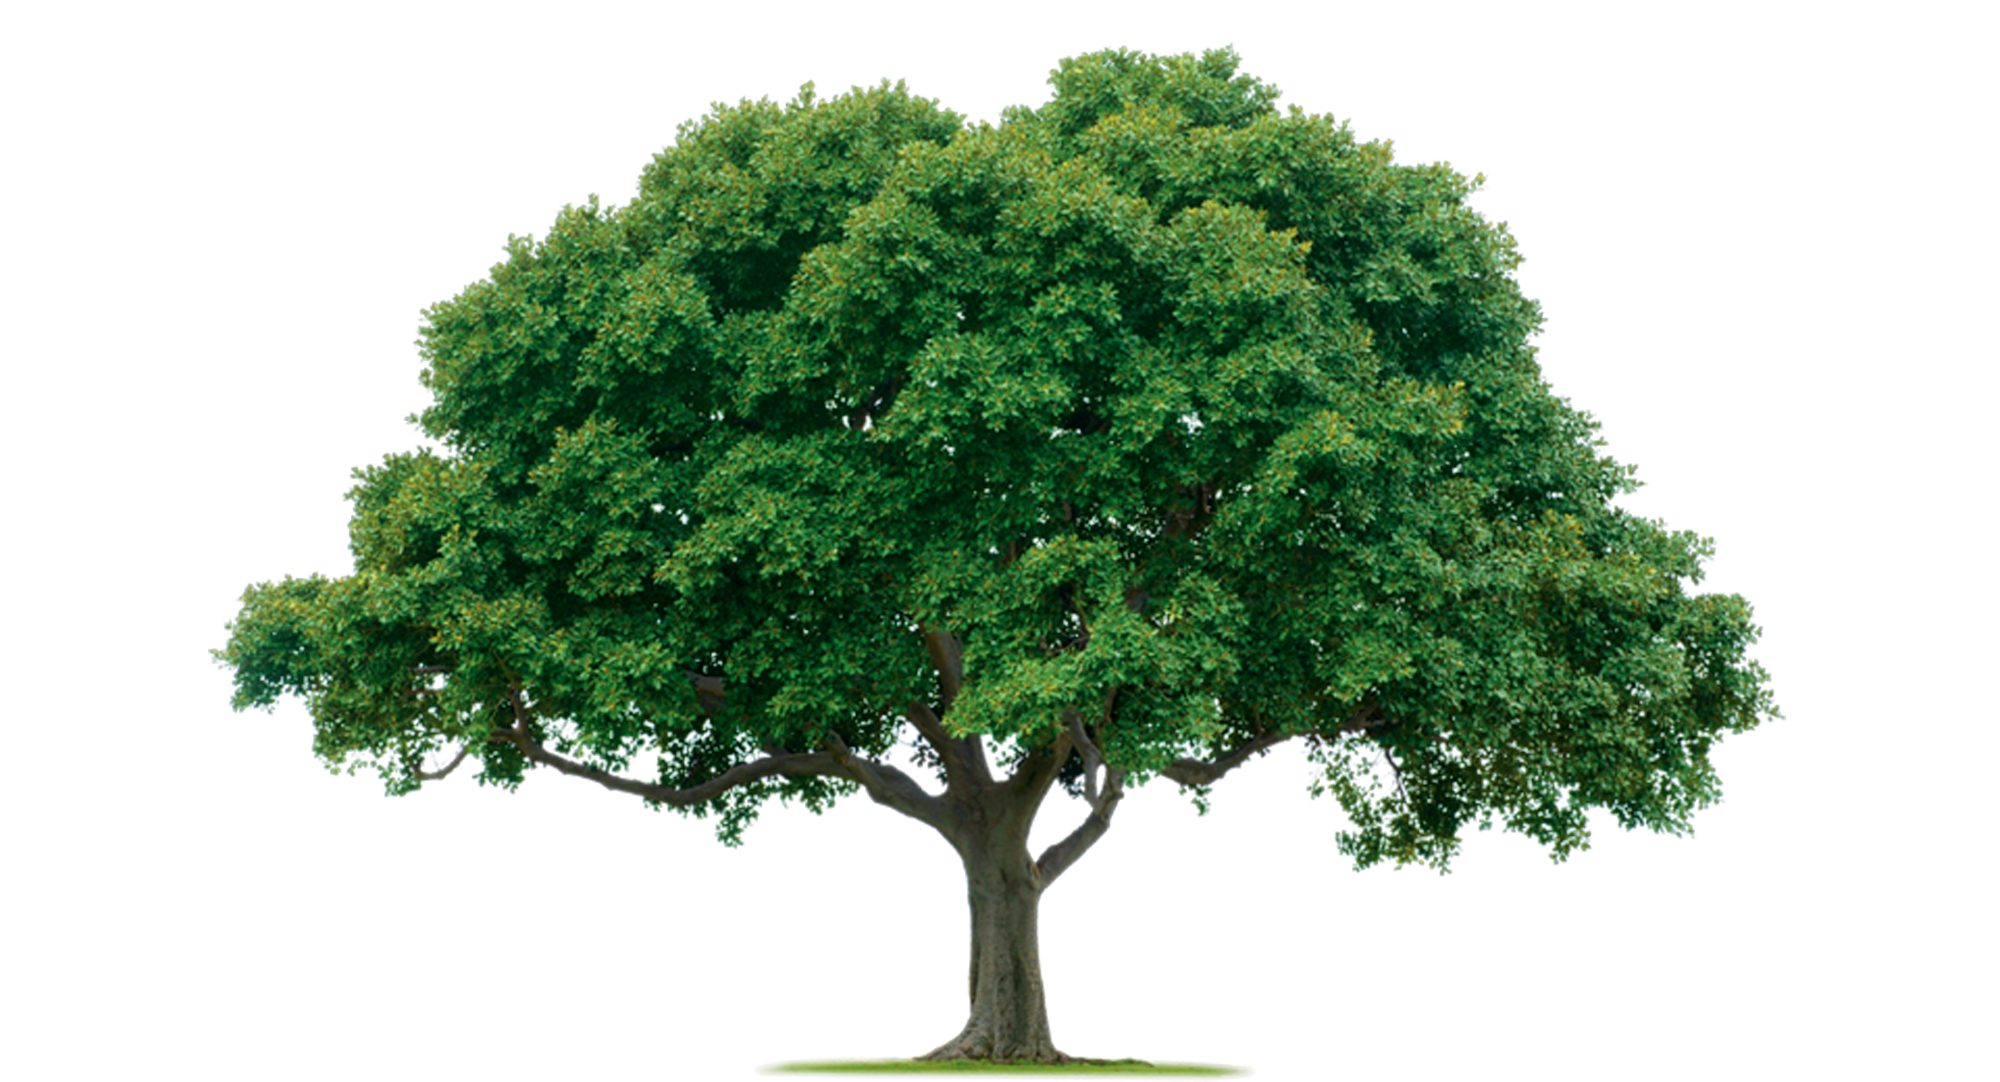
\includegraphics[scale=.15]{tree2.png}
\end{center}

Para imágenes en color se utilizan tres matrices con tonalidades RGB (red, green, blue), pero vamos a utilizar solo tonalidades de gris, tomamos $\Ab \in \R^{1080 \times 2000}$.

\begin{center}
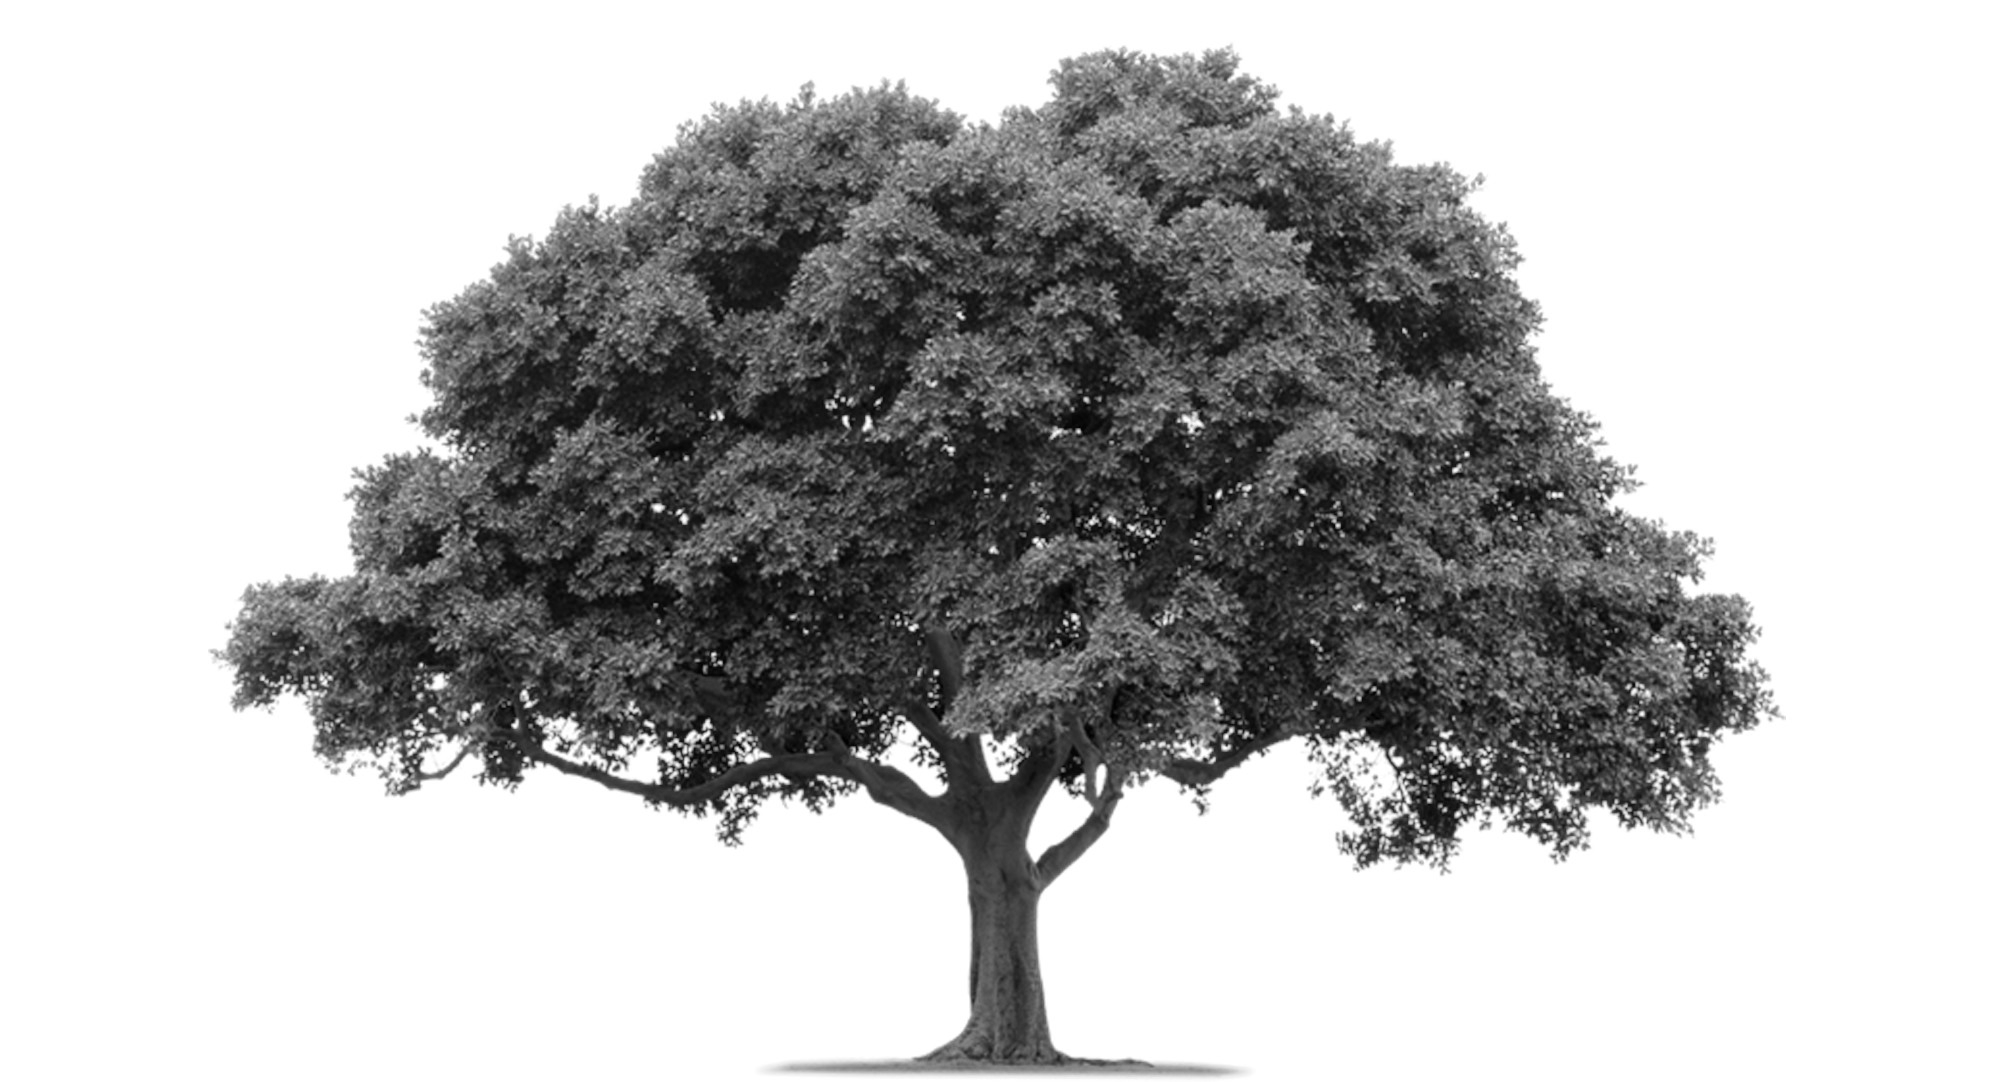
\includegraphics[scale=.15]{grayTree.png}
\end{center}

Calculamos la descomposición $\Ab = \Ub \Sigmab \Vb^*$ y graficamos los logartimos de los valores singulares. Podemos tomar los primeros 987 valores singulares sin casi perder información, pero no es suficiente compresión.

\begin{center}
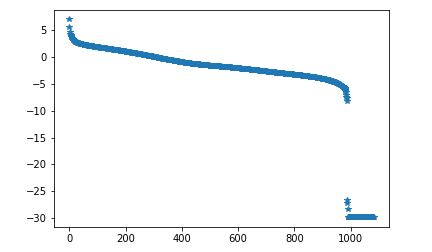
\includegraphics[scale = 0.6]{logS2.png}
\end{center}

Probamos tomar las primeros 200 valores singulares. Es decir, tomamos
$$\tilde \Ab = \underset{1080 \times 200}{\tilde \Ub} \quad
\underset{200 \times 200} {\tilde \Sigmab} \quad
\underset{200 \times 2000}{\tilde \Vb^*}
$$
y obtenemos la imagen
\begin{center}
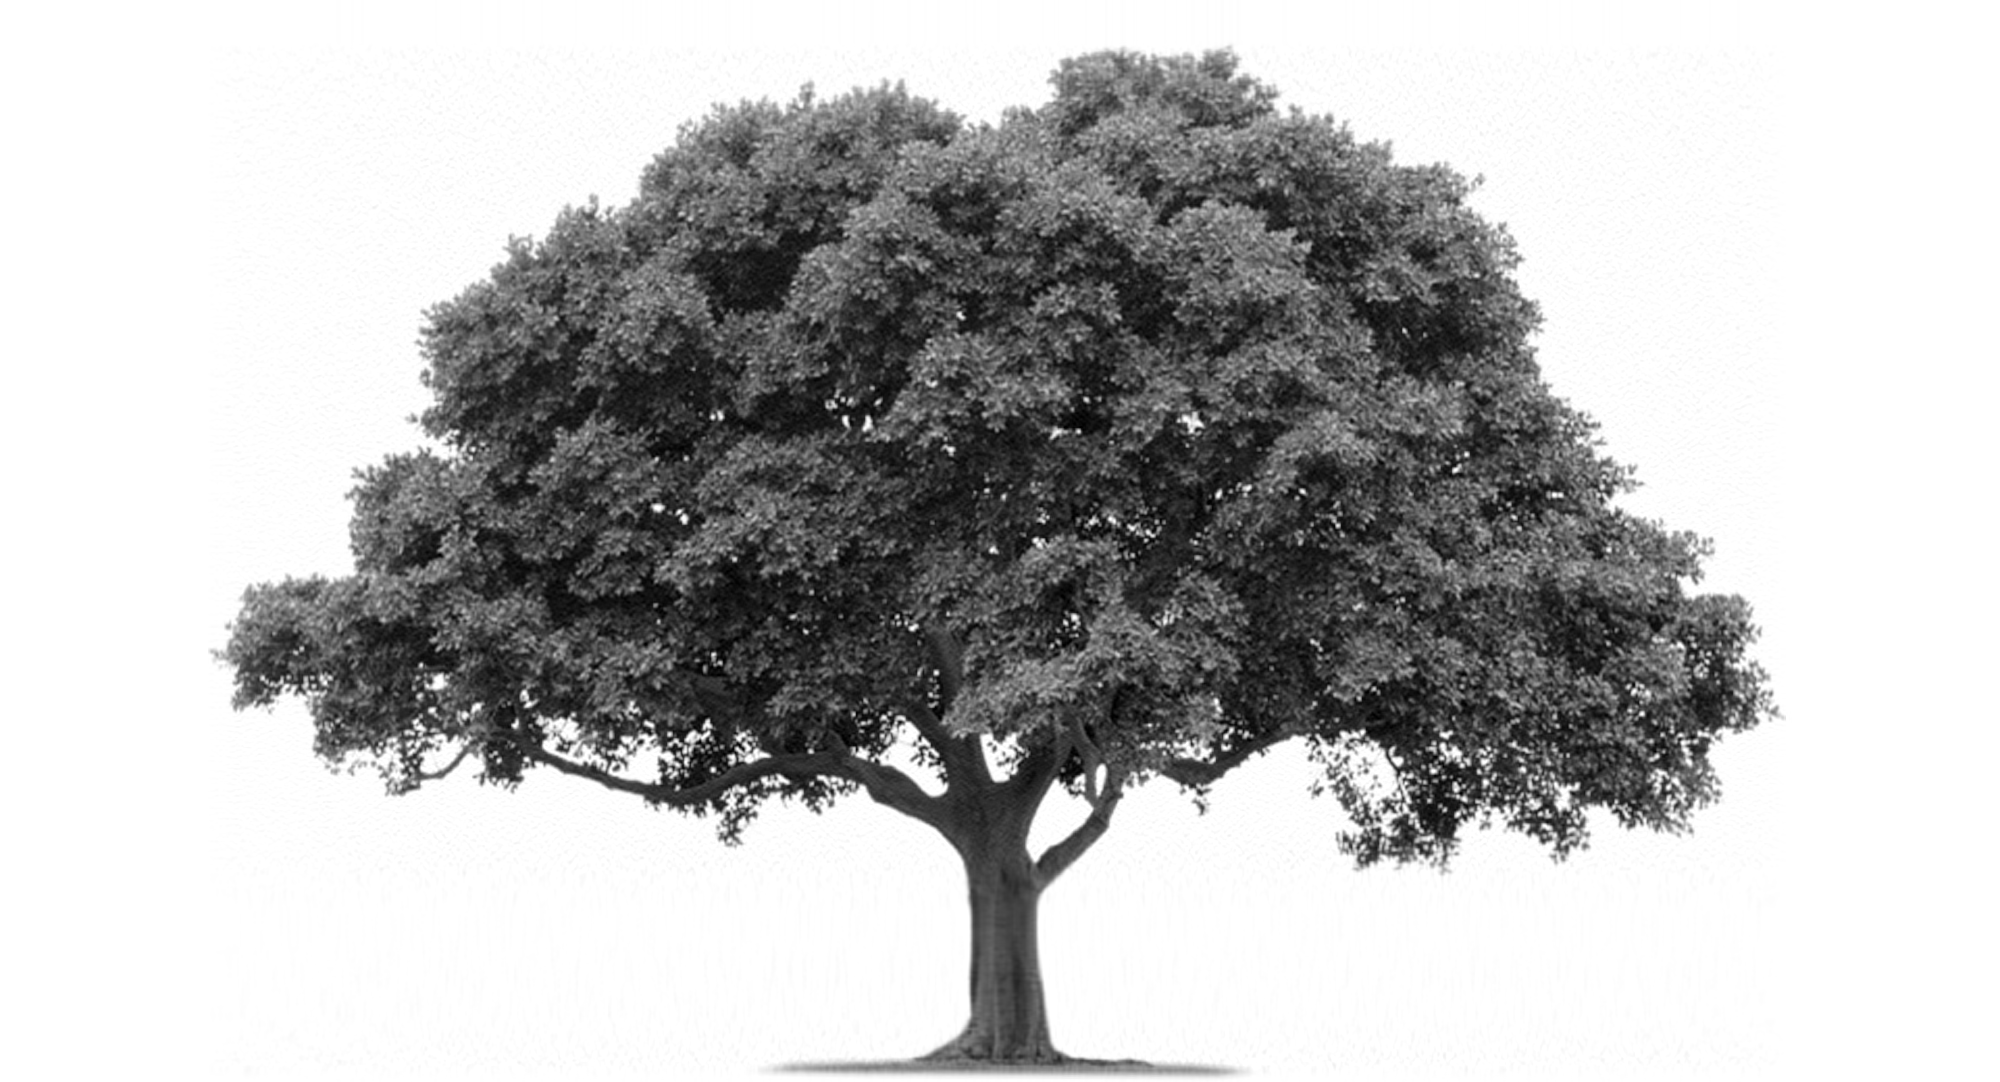
\includegraphics[scale = .12]{grayTree200.png}
\end{center}

\end{ejemplo}

\begin{ejercicio} 
Calcular el porcentaje de compresión (es decir, la relación entre la cantidad de números que guardamos para la imagen comprimida y la cantidad de números de la imagen original).
\end{ejercicio}


